\section{Coupled water flow and contaminant transport}
%----------------------------------------------------------------------------------------
%	INTRODUCTION
%----------------------------------------------------------------------------------------
\subsection{Goal and Complexity}
\subsection*{Complexity: Medium}

\subsection*{Prerequisites: None}

The goal of this tutorial is to introduce contaminant transport. For this we couple the $DRUtES$ standard Richards equation module with the ADE module. ADE stands for Advection-Dispersion-Equation. The advection will be calculated through the Richards-Equation (water flow).

\begin{figure}[!h]
\centering
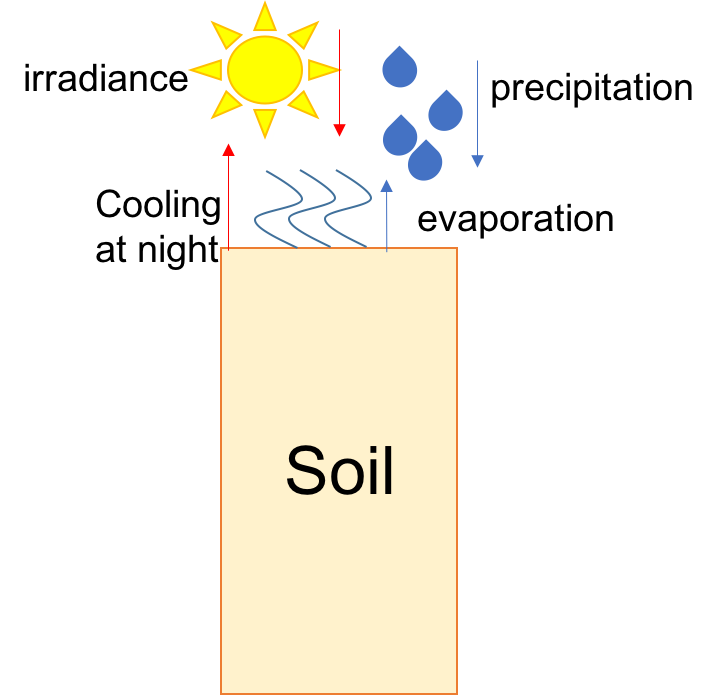
\includegraphics[width=8cm]{Fig_coupledade/coupled.png}
\caption{Simplified scheme of coupled model.}
\end{figure}

In this example we assume that the contaminant is soluble and in the water. No adsorption or desorption occurs. 

In this tutorial five configuration files will be modified step by step. All configuration files are located in the folder \emph{drutes.conf} and respective subfolders. \begin{enumerate}
\item For selection of the module, dimension and time information we require \emph{global.conf}.  \emph{global.conf} is located in \emph{drutes.conf / global.conf}. 
\item To define the mesh or spatial discretization in 1D,  we require \emph{drumesh1D.conf}. \emph{drumesh1D.conf} is located in \emph{drutes.conf / mesh / drumesh1D.conf}. 
\item To define the precipitation, we require \emph{matrix.conf}. \emph{matrix.conf} is located in \emph{drutes.conf /water.conf/ matrix.conf}. 
\item To select the ADE module and link it to the water module, we require \emph{ADE.conf}. \emph{ADE.conf} is located in \emph{drutes.conf /ADE/ ADE.conf}. 
\item To define the contaminant transport, we require \emph{contaminant.conf}. \emph{contaminant.conf} is located in \emph{drutes.conf /ADE/ contaminant.conf}. 
\end{enumerate}
$DRUtES$ works with configuration input file with the file extension .conf. Blank lines and lines starting with \# are ignored. The input mentioned in this tutorial therefore needs to be placed one line below the mentioned keyword, unless stated otherwise. 

\newpage
\subsection{Scenarios}

We are using the well-known van Genuchten-Mualem parameterization to describe the soil hydraulic properties of our soils and contaminant transport. 

\begin{table}[!h]
\centering
\caption{\label{tab_heat}Material properties needed for scenarios.}
\adjustbox{max height=\dimexpr\textheight-2cm\relax,
           max width=\textwidth}{

\small\begin{tabular}{l l c c c }
\hline
Parameter & Description & Sand & Clay & Contaminant\\
\hline

$\alpha$ [cm$^{-1}$]& inverse of the air entry value &0.05 & 0.01 \\
 $n$ [-]& shape parameter &2 & 1.4\\
 $m$ [-]& shape parameter &0.5 & 0.2857  \\
  $ \theta_s$ [-]&saturated vol. water content&0.45 &0.45 \\
  $ \theta_r$ [-]& residual vol. water content&0.05 &0.05  \\
  $Ss$ [cm$^{-1}$] & specific storage & 0 & 0 \\
  $K_s$ [cm d$^{-1}$] & saturated hydraulic conductivity & 100 & 1\\ 
  D [cm$^{2}$ d$^{-1}$] & diffusion  &10e-3& 10e-3 \\
  D$_v$ [cm ] & dispersivity  & 30 & 100	 \\ 
 c$_\mathrm{init}$ [mg cm$^{-3}$] & initial concentration & & & 2\\
\hline
\end{tabular}
}
\end{table}

The domain scheme is shown in Fig. \ref{domain}. We need to define 4 boundary conditions. Our mesh requires 5 different layers to accomodate for the contaminantion, the extra soil and the layers in between.

\begin{figure}[!h]
\centering
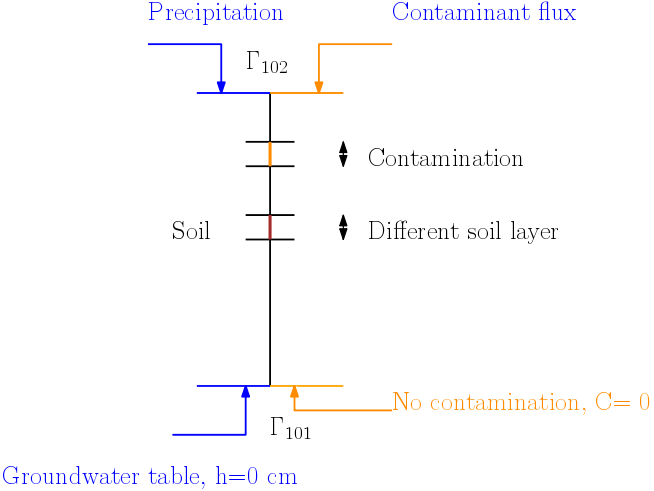
\includegraphics[width=10cm]{Fig_coupledade/domain_set_upADEwater.png}
\caption{\label{domain}1D domain set-up of coupled scenario with top and bottom boundary conditions. There are now two boundary condtions at the top and two boundary conditions at the bottom: contaminant transport and water flow. The top boundary is defined by the interactions with the atmosphere and the bottom boundary is defined by the constant groundwater table.}
\end{figure}

\section*{Scenario 1}

We first assume that the soil is homogeneous.

$global.conf$: Choose correct model, dimension, time discretization and observation times.
\begin{enumerate}
\item Open \textbf{\emph{global.conf}} in a text editor of your choice. 
\item Model type: Your first input is the module. Input is \textbf{ADE}.
\item Initial mesh configuration \begin{enumerate}
\item The dimension of our problem is 1. Input: 1.
\item We use the internal mesh generator. Input: 1. 
\end{enumerate}
\item Error criterion \begin{enumerate} 
\item Maximum number of iteration of the Picard method: 20 
\item h tolerance: 1e-3.
\end{enumerate}
\item Time information 
\begin{enumerate} 
%\item integration method is 3 point formula. Input: 30. 
\item Time units are in hours: input d
\item Initial time: 1e-4.
\item End time: 10.
\item Minimum time step: 1e-12.
\item Maximum time step: 0.005.
\end{enumerate}
\item Observation time settings \begin{enumerate}
\item Observation time method: 2
\item Set file format of observation: pure. Output in 1D is always in raw data. Different options will not impact output in 1D.
\item Make sequence of observation time: n
\item Number of observation times: 9
\item Observation time values: 1, 2, 3,4,5,6,7,8,9. Use a new line for each input. \textit{DRUtES} will generate 11 output files for each modeled component, e.g.\textit{RE\_matrix\_press\_head-x.dat}, where x is the ID of the observation point. The initial and final time value will be automatically be printed.
\end{enumerate}
\item Observation point settings \begin{enumerate}
\item Number of observation points: 6 
\item Observation point coordinates: 200, 195,187.5,182.5,175, 150. Use a new line for each input. \textit{DRUtES} will generate 6 output files for each modeled component, e.g. \textit{obspt\_RE\_matrix-1.out}, where x is the ID of the observation point. 
\end{enumerate}
\item Ignore other settings for now. 
\item Save $global.conf$
\end{enumerate}


$drumesh1D.conf$: Mesh definition, i.e. number of materials and spatial discretization
\begin{enumerate}
\item Open \textbf{\emph{drumesh1D.conf}} in a text editor of your choice. 
\item Geometry information: 200 cm - domain length
\item Amount of intervals: 1
\item
\adjustbox{max height=\dimexpr\textheight-5cm\relax,
           max width=\textwidth}{
\small\begin{tabular}{|c | c | c|}
\hline
density & bottom & top \\
 \hline
4 & 0 & 200\\
\hline
\end{tabular}
}
\item number of materials: 5
\item \adjustbox{max height=\dimexpr\textheight-5cm\relax,
           max width=\textwidth}{
\small\begin{tabular}{|c | c | c|}
\hline
id & bottom & top \\
 \hline
1   &     0         & 170 \\
2   &     170      &  180 \\
3   &     180     &   185 \\
4    &    185     &   190 \\
5    &    190    &    200 \\
\hline
\end{tabular}
}
\item Save $drumesh1D.conf$
\end{enumerate}

\emph{matrix.conf}: Configuration file for water flow 


\begin{enumerate}
\item Open \emph{matrix.conf} in a text editor of your choice. 
\item How-to use constitutive relations? [integer]: 1
\item Length of interval for precalculating the constitutive functions: 200
\item Discretization step for constituitive function precalculation: 0.1
\item number of soil layers [integer]: 5
\item \adjustbox{max height=\dimexpr\textheight-5cm\relax,
	max width=\textwidth}{
	\small\begin{tabular}{|c | c | c|c | c | c|}
		\hline
		alpha & n & m & theta\_r & theta\_s & specific storage\\
		\hline
		0.05 & 2  & 0.5 & 0.05 & 0.45  &0  \\
			0.05 & 2  & 0.5 & 0.05 & 0.45  &0  \\
				0.05 & 2  & 0.5 & 0.05 & 0.45  &0  \\
					0.05 & 2  & 0.5 & 0.05 & 0.45  &0  \\
						0.05 & 2  & 0.5 & 0.05 & 0.45  &0  \\
		\hline
	\end{tabular}
}
\item The angle of the anisotropy determines the angle of the reference coordinate system. 0 means vertical flow. Anisotropy description. Anisotpropy description and hydraulic conductivity\\ \adjustbox{max height=\dimexpr\textheight-5cm\relax,
	max width=\textwidth}{
	\small\begin{tabular}{|c | c |}
		\hline
		angle [degrees] & K\_11  \\
		\hline
		0 & 100  \\
		0 & 100  \\
		0 & 100  \\
		0 & 100  \\
		0 & 100  \\
		\hline
	\end{tabular}
}
\item sink(-) /source (+) term per layer: \\ 0 \\ 0 \\0 \\0 \\ 0
\item Initial condition is a constant pressure head of -200 cm across the soil. \adjustbox{max height=\dimexpr\textheight-5cm\relax,
	max width=\textwidth}{
	\small\begin{tabular}{|c | c | c|c |}
		\hline
		 init. cond [real] & type of init. cond &RCZA method [y/n] &  RCZA method val.  \\
		\hline
		   0.0           &            H\_tot                      & n		   &          0 \\
		   		   0.0           &            H\_tot                      & n		   &          0 \\
		   		   		   0.0           &            H\_tot                      & n		   &          0 \\
		   		   		   		   0.0           &            H\_tot                      & n		   &          0 \\
		   		   		   		   		   0.0           &            H\_tot                      & n		   &          0 \\
		\hline
	\end{tabular}
}
\item number of boundaries: 2
\item \adjustbox{max height=\dimexpr\textheight-5cm\relax,
	max width=\textwidth}{
	\small\begin{tabular}{|c | c | c|c |}
		\hline
		boundary ID& boundary type   & use rain.dat [y/n]   & value  \\
		\hline
	101    &                   1        &           n        &        0.0 \\
	102             &          2         &          n         &       0.5        \\
	
		\hline
	\end{tabular}
}
\item Save matrix.conf.
\end{enumerate}

Contaminant transport 
\emph{ADE.conf}

\begin{enumerate}
\item Open \emph{ADE.conf} in a text editor of your choice. 
\item specify coupling with Richards equation [y/n]: y
\item use sorption: n 
\item Save ADE.conf.
\end{enumerate}

\emph{contaminant.conf}

\begin{enumerate}
	\item Open \emph{contaminant.conf} in a text editor of your choice. 
	\item number of layers: 5
	\item molecular diffusion: \\ 10e-3 \\ 10e-3 \\ 10e-3 \\ 10e-3 \\ 10e-3
	\item dispersivity: \\ \adjustbox{max height=\dimexpr\textheight-5cm\relax,
		max width=\textwidth}{
		\small\begin{tabular}{|c | c |}
			\hline
			angle [degrees] & D\_11  \\
			\hline
			0 & 30  \\
			0 & 30  \\
			0 & 30  \\
			0 & 30  \\
			0 & 30  \\
			\hline
		\end{tabular}
	}
	\item initial condition: \\ \adjustbox{max height=\dimexpr\textheight-5cm\relax,
		max width=\textwidth}{
		\small\begin{tabular}{|c | c |}
			\hline
			value & type  \\
			\hline
			0 & ca  \\
			0 & ca  \\
			0 & ca  \\
			2 & ca  \\
			0 & ca  \\
			\hline
		\end{tabular}
	}
	\item number of different orders of reactions: 1
	\item orders of reaction: \\ 1 \\ 1 \\ 1 \\ 1 \\ 1
	\item reaction coefficients: \\0 \\0\\0\\0\\0 
	\item number of boundaries: 2
	\item \adjustbox{max height=\dimexpr\textheight-5cm\relax,
		max width=\textwidth}{
		\small\begin{tabular}{|c | c | c|c |}
			\hline
			boundary ID& boundary type   & use rain.dat [y/n]   & value  \\
			\hline
			101    &                   1        &           n        &        0.0 \\
			102             &          2         &          n         &       0.0        \\
			
			\hline
		\end{tabular}
	}
\item save $contaminant.conf$
\end{enumerate}

\section*{Run scenario 1}
Run the simulation in the terminal console.
\begin{enumerate}
\item Make sure you are in the right directory. 
\item To execute $DRUtES$: \\
\$ bin/drutes
\item After the simulation finishes, to generate png plots execute provided R script: \\
\$ Rscript drutes.conf/makeplot.R -name coupled\_samesoil \\
\item The output of the simulation can be found in the folder out
\end{enumerate}

\section*{Scenario 2}

In scenario 2 we introduce a clay layer in depth 170-180 cm. For this, we need to change matrix.conf and contaminant.conf. \\

Changes in matrix.conf 

\begin{enumerate}
	\item Change the 2nd van Genuchten parameter set: \\ \adjustbox{max height=\dimexpr\textheight-5cm\relax,
		max width=\textwidth}{
		\small\begin{tabular}{|c | c | c|c | c | c|}
			\hline
			alpha & n & m & theta\_r & theta\_s & specific storage\\
			\hline
			0.05 & 2  & 0.5 & 0.05 & 0.45  &0  \\
			0.01 & 1.4  & 0.2857 & 0.05 & 0.45  &0  \\
			0.05 & 2  & 0.5 & 0.05 & 0.45  &0  \\
			0.05 & 2  & 0.5 & 0.05 & 0.45  &0  \\
			0.05 & 2  & 0.5 & 0.05 & 0.45  &0  \\
			\hline
		\end{tabular}
	}
	\item Change the 2nd hydraulic conductivity. The angle of the anisotropy determines the angle of the reference coordinate system. 0 means vertical flow. Anisotropy description. Anisotpropy description and hydraulic conductivity\\ \adjustbox{max height=\dimexpr\textheight-5cm\relax,
		max width=\textwidth}{
		\small\begin{tabular}{|c | c |}
			\hline
			angle [degrees] & K\_11  \\
			\hline
			0 & 100  \\
			0 & 1  \\
			0 & 100  \\
			0 & 100  \\
			0 & 100  \\
			\hline
		\end{tabular}
	}
	\item save $matrix.conf$
\end{enumerate}

Changes in contaminant.conf
\begin{enumerate}
	\item Change the second dispersivity value to 100.
		dispersivity: \\ \adjustbox{max height=\dimexpr\textheight-5cm\relax,
			max width=\textwidth}{
			\small\begin{tabular}{|c | c |}
				\hline
				angle [degrees] & D\_11  \\
				\hline
				0 & 30  \\
				0 & 100  \\
				0 & 30  \\
				0 & 30  \\
				0 & 30  \\
				\hline
			\end{tabular}
		}
	\item save contaminant.conf
\end{enumerate}


\section*{Run scenario 2}
Run the simulation in the terminal console.
\begin{enumerate}
	\item Make sure you are in the right directory. 
	\item To execute $DRUtES$: \\
	\$ bin/drutes
	\item After the simulation finishes, to generate png plots execute provided R script: \\
	\$ Rscript drutes.conf/makeplot.R -name coupled\_claylense \\
	\item The output of the simulation can be found in the folder out
\end{enumerate}


\section*{Tasks}

\begin{enumerate}
\item Describe the distribution of the contaminant without and with the clay layer.
\item Investigate how the simulation differs: (i) With a different soil material (ii) when you include a reaction in contaminant.confS
\end{enumerate}

\newpage

\section*{Simulation Results}

The simulation nicely shows how the contamination moves downwards into the soil and disperses to compensate for concentration differences. The clay layer hinders the water flow into deeper layers and therefore also the advection. Due to the high dispersion in the clay layer the contaminant concentration becomes more evenly distributed in that layer. 


\begin{figure}[!h]
	\centering
	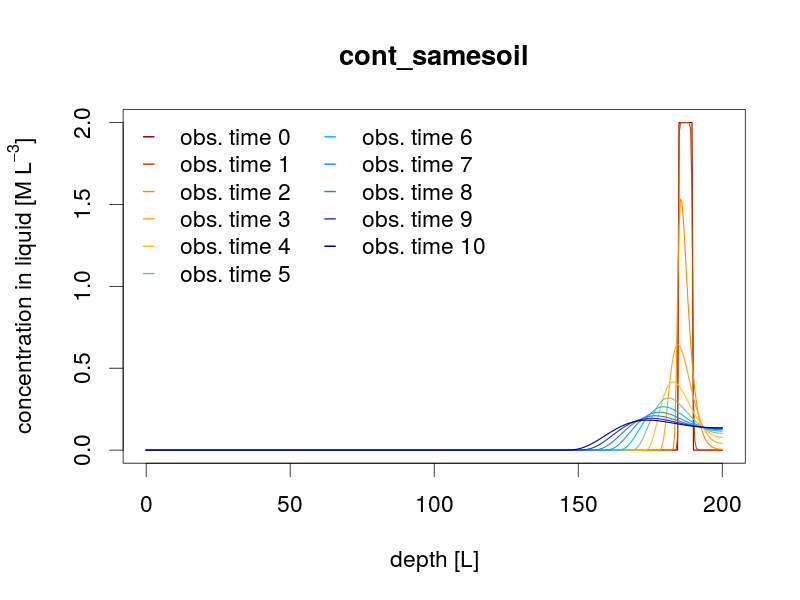
\includegraphics[width=6cm]{Fig_coupledade/obs_conta_cont_samesoil.png}
	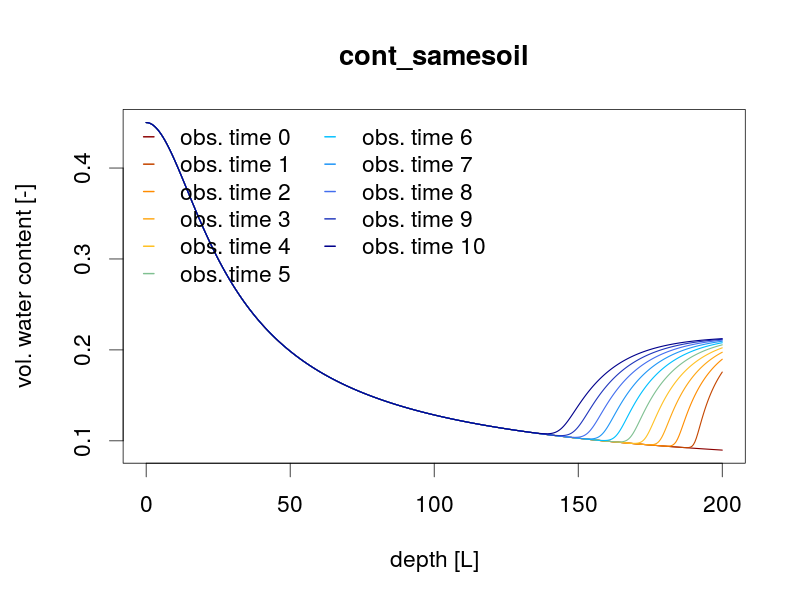
\includegraphics[width=6cm]{Fig_coupledade/obs_water_cont_samesoil.png}
	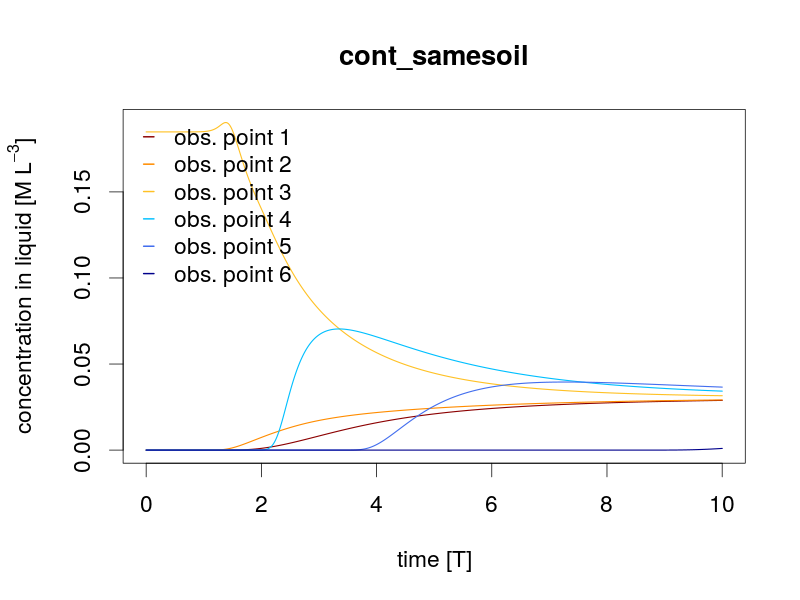
\includegraphics[width=6cm]{Fig_coupledade/obs_conc_point_cont_samesoil.png}
	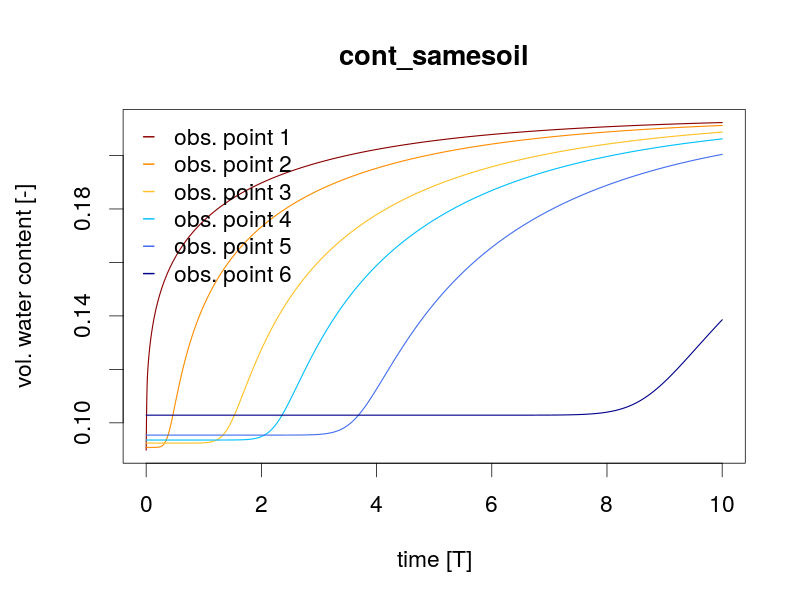
\includegraphics[width=6cm]{Fig_coupledade/obs_water_point_cont_samesoil.png}
	\caption{Water content  and contaminant concentration at the observation points and observation times the homogeneous soil.}
\end{figure}

\begin{figure}[!h]
	\centering
	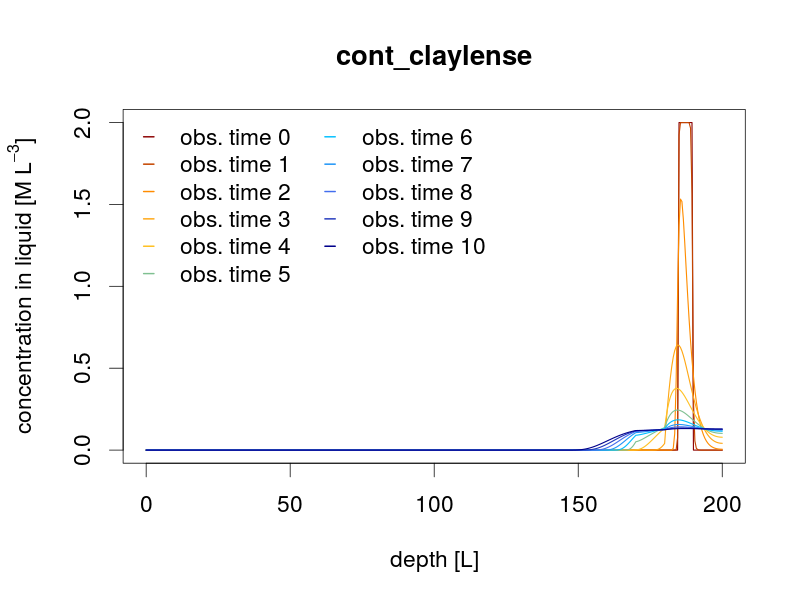
\includegraphics[width=6cm]{Fig_coupledade/obs_conta_cont_claylense.png}
	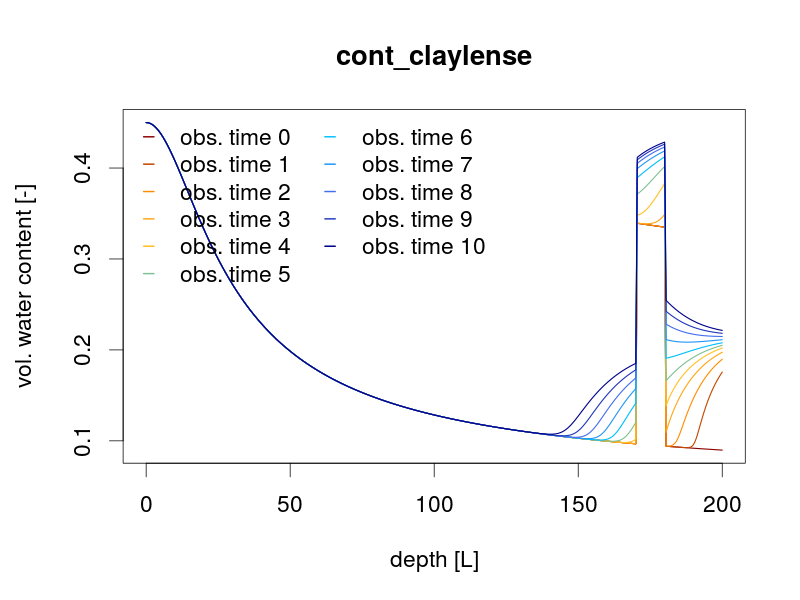
\includegraphics[width=6cm]{Fig_coupledade/obs_water_cont_claylense.png}
	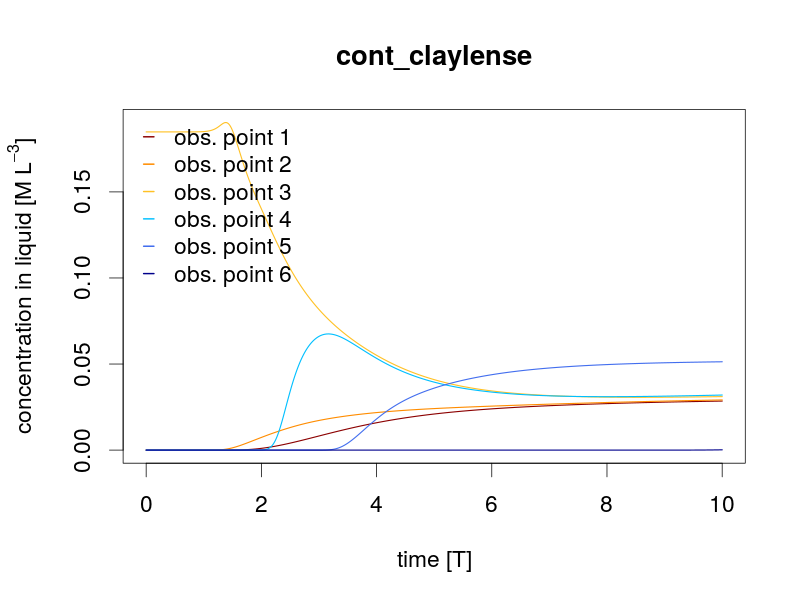
\includegraphics[width=6cm]{Fig_coupledade/obs_conc_point_cont_claylense.png}
	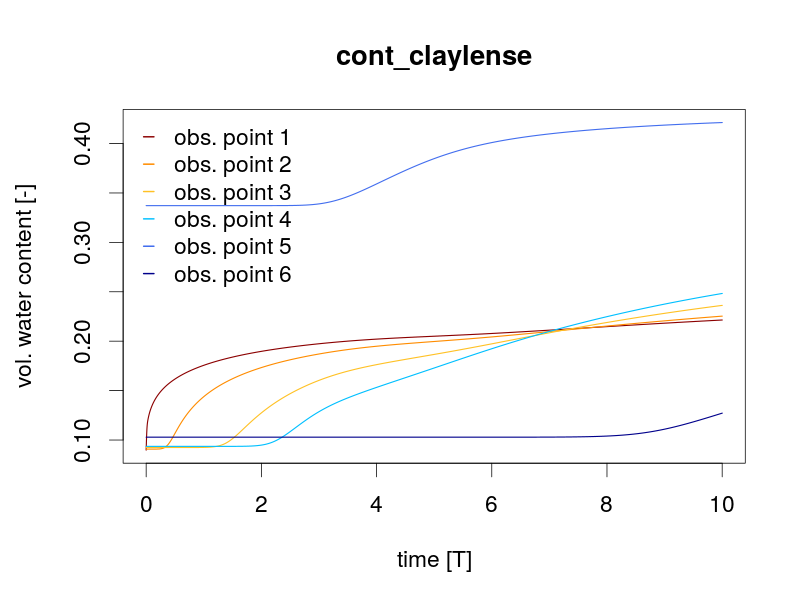
\includegraphics[width=6cm]{Fig_coupledade/obs_water_point_cont_claylense.png}
	\caption{Water content  and contaminant concentration at the observation points and observation times with a clay layer.}
\end{figure}


\newpage
\newpage
\newpage
\newpage
\pagebreak
\subsection{Outcome}
\begin{enumerate}
\item You got familiar with simple contaminant transport.
\item You simulated coupled water flow and contamination transport.
\item You understand the difference between advection and dispersion.
\end{enumerate}
